\section{Proceso de desarrollo}
El módulo como proyecto de desarrollo enfocado a la metodología Ágil se encuentra dividido en varias épicas para partir en las funcionalidades.

Una épica se encuentra dividida en varias historias de usuario, donde las historias de usuario tienen el propósito de entregar valores de negocio al cliente en un periodo establecido de 2 semanas como sprint. Estas historias de usuario pueden ser a la vez divididas buscando la simplicidad de las historias donde cada una debe seguir la práctica INVEST de la metodología Ágil.

Cada historia puede estar compuesta de tareas que tienen como propósito servir al desarrollador como recordatorio de algunas labores pendientes a la hora de desarrollar la historia. Cada tarea debía tener un encargado, pero no necesariamente una persona trabajando en dicha tarea.

% \begin{figure}[H]
% \centering
% 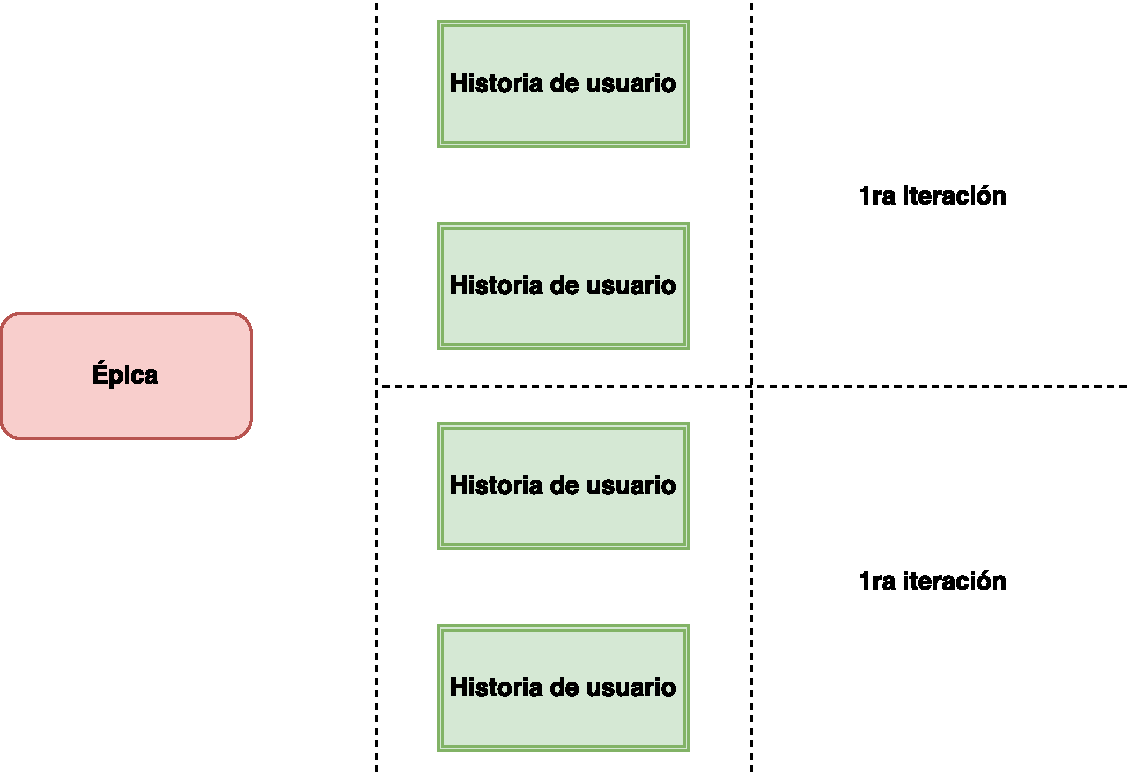
\includegraphics[width=125mm,scale=1]{Capitulos/PropuestadeSolucion/Imagenes/epic_diagram}
% \caption{Diagrama de definición de épicas en la metodología ágil}
%   \label{epic}
% \end{figure}

El PO\footnote{de sus siglas en inglés, Product Owner, que significa en español dueño del producto.} se encarga de la creación de épicas e historias de usuario, en caso de que la historia sea muy grande para terminar en un solo sprint o iteración se vuelve a partir en historias más pequeñas. 

Para el caso de estudio, cada sprint consta de 2 semanas de trabajo, donde los desarrolladores como equipo se comprometen a entregar cierto valor de negocio que ellos estiman poder terminar en dicho periodo. Sin embargo, en caso de que el equipo considere que la totalidad de historias no podrán ser entregadas antes de que termine el periodo se pasa al siguiente sprint o se achica la historia minimizando los criterios de aceptación y los restantes se agregan en otra historia de usuario para las siguientes iteraciones.

Cada equipo tiene un líder, donde cada líder tiene como rol ser la brecha que une al PO con los desarrolladores. El PO se reúne con el líder de cada equipo para verificar las prioridades de las historias de usuario que están pendientes en el backlog\footnote{Bolsa de historias de usuarios pendientes.}. 

Al inicio del diseño de la aplicación se llevará a cabo una serie de diseños de funcionalidad y usabilidad que llevar a la mejor experiencia de uso del módulo de gestión curricular, donde dichos diseños serán validados por el equipo en los Estados Unidos antes de iniciar el desarrollo.

Se ha utilizado la técnica Scrum en la gestión de proyectos ágiles debido a que en la misma se aplican de manera regular un conjunto de prácticas para trabajar colaborativamente, en equipo, y obtener el mejor resultado posible de un proyecto, además de que el equipo ya se encontraba familiarizado por la misma. Estas prácticas se apoyan unas a otras y su selección tiene origen en un estudio de la manera de trabajar de equipos altamente productivos.

Se realizan entregas parciales y regulares del producto final, priorizadas por el beneficio que aportan al PO. Por ello, Scrum está especialmente indicado para proyectos en entornos complejos donde se necesita obtener resultados con el mínimo esfuerzo y los requisitos son cambiantes o poco definidos. Además, en dichos ambientes la innovación, la competitividad, la flexibilidad, y la productividad son fundamentales.

\subsection{Proceso}
Como ya se mencionó, el proyecto se ejecutó en bloques temporales cortos y fijos que los conocemos como sprints o iteraciones. Estas iteraciones por lo general duran 2 semanas aunque en algunos equipos son de 3 y hasta 4 semanas, límite máximo de feedback y reflexión \citep{davis_agile_2015}. Cada iteración tiene que proporcionar un resultado completo, un incremento de producto final que sea susceptible de ser entregado con el mínimo esfuerzo al cliente cuando lo solicite.

El proceso parte de la lista de objetivos o requisitos priorizada del producto, que actúa como plan del proyecto. En esta lista el cliente prioriza los objetivos balanceando el valor que le aportan respecto a su coste y quedan repartidos en sprints y entregas.

% \begin{figure}[H]
% \centering
% 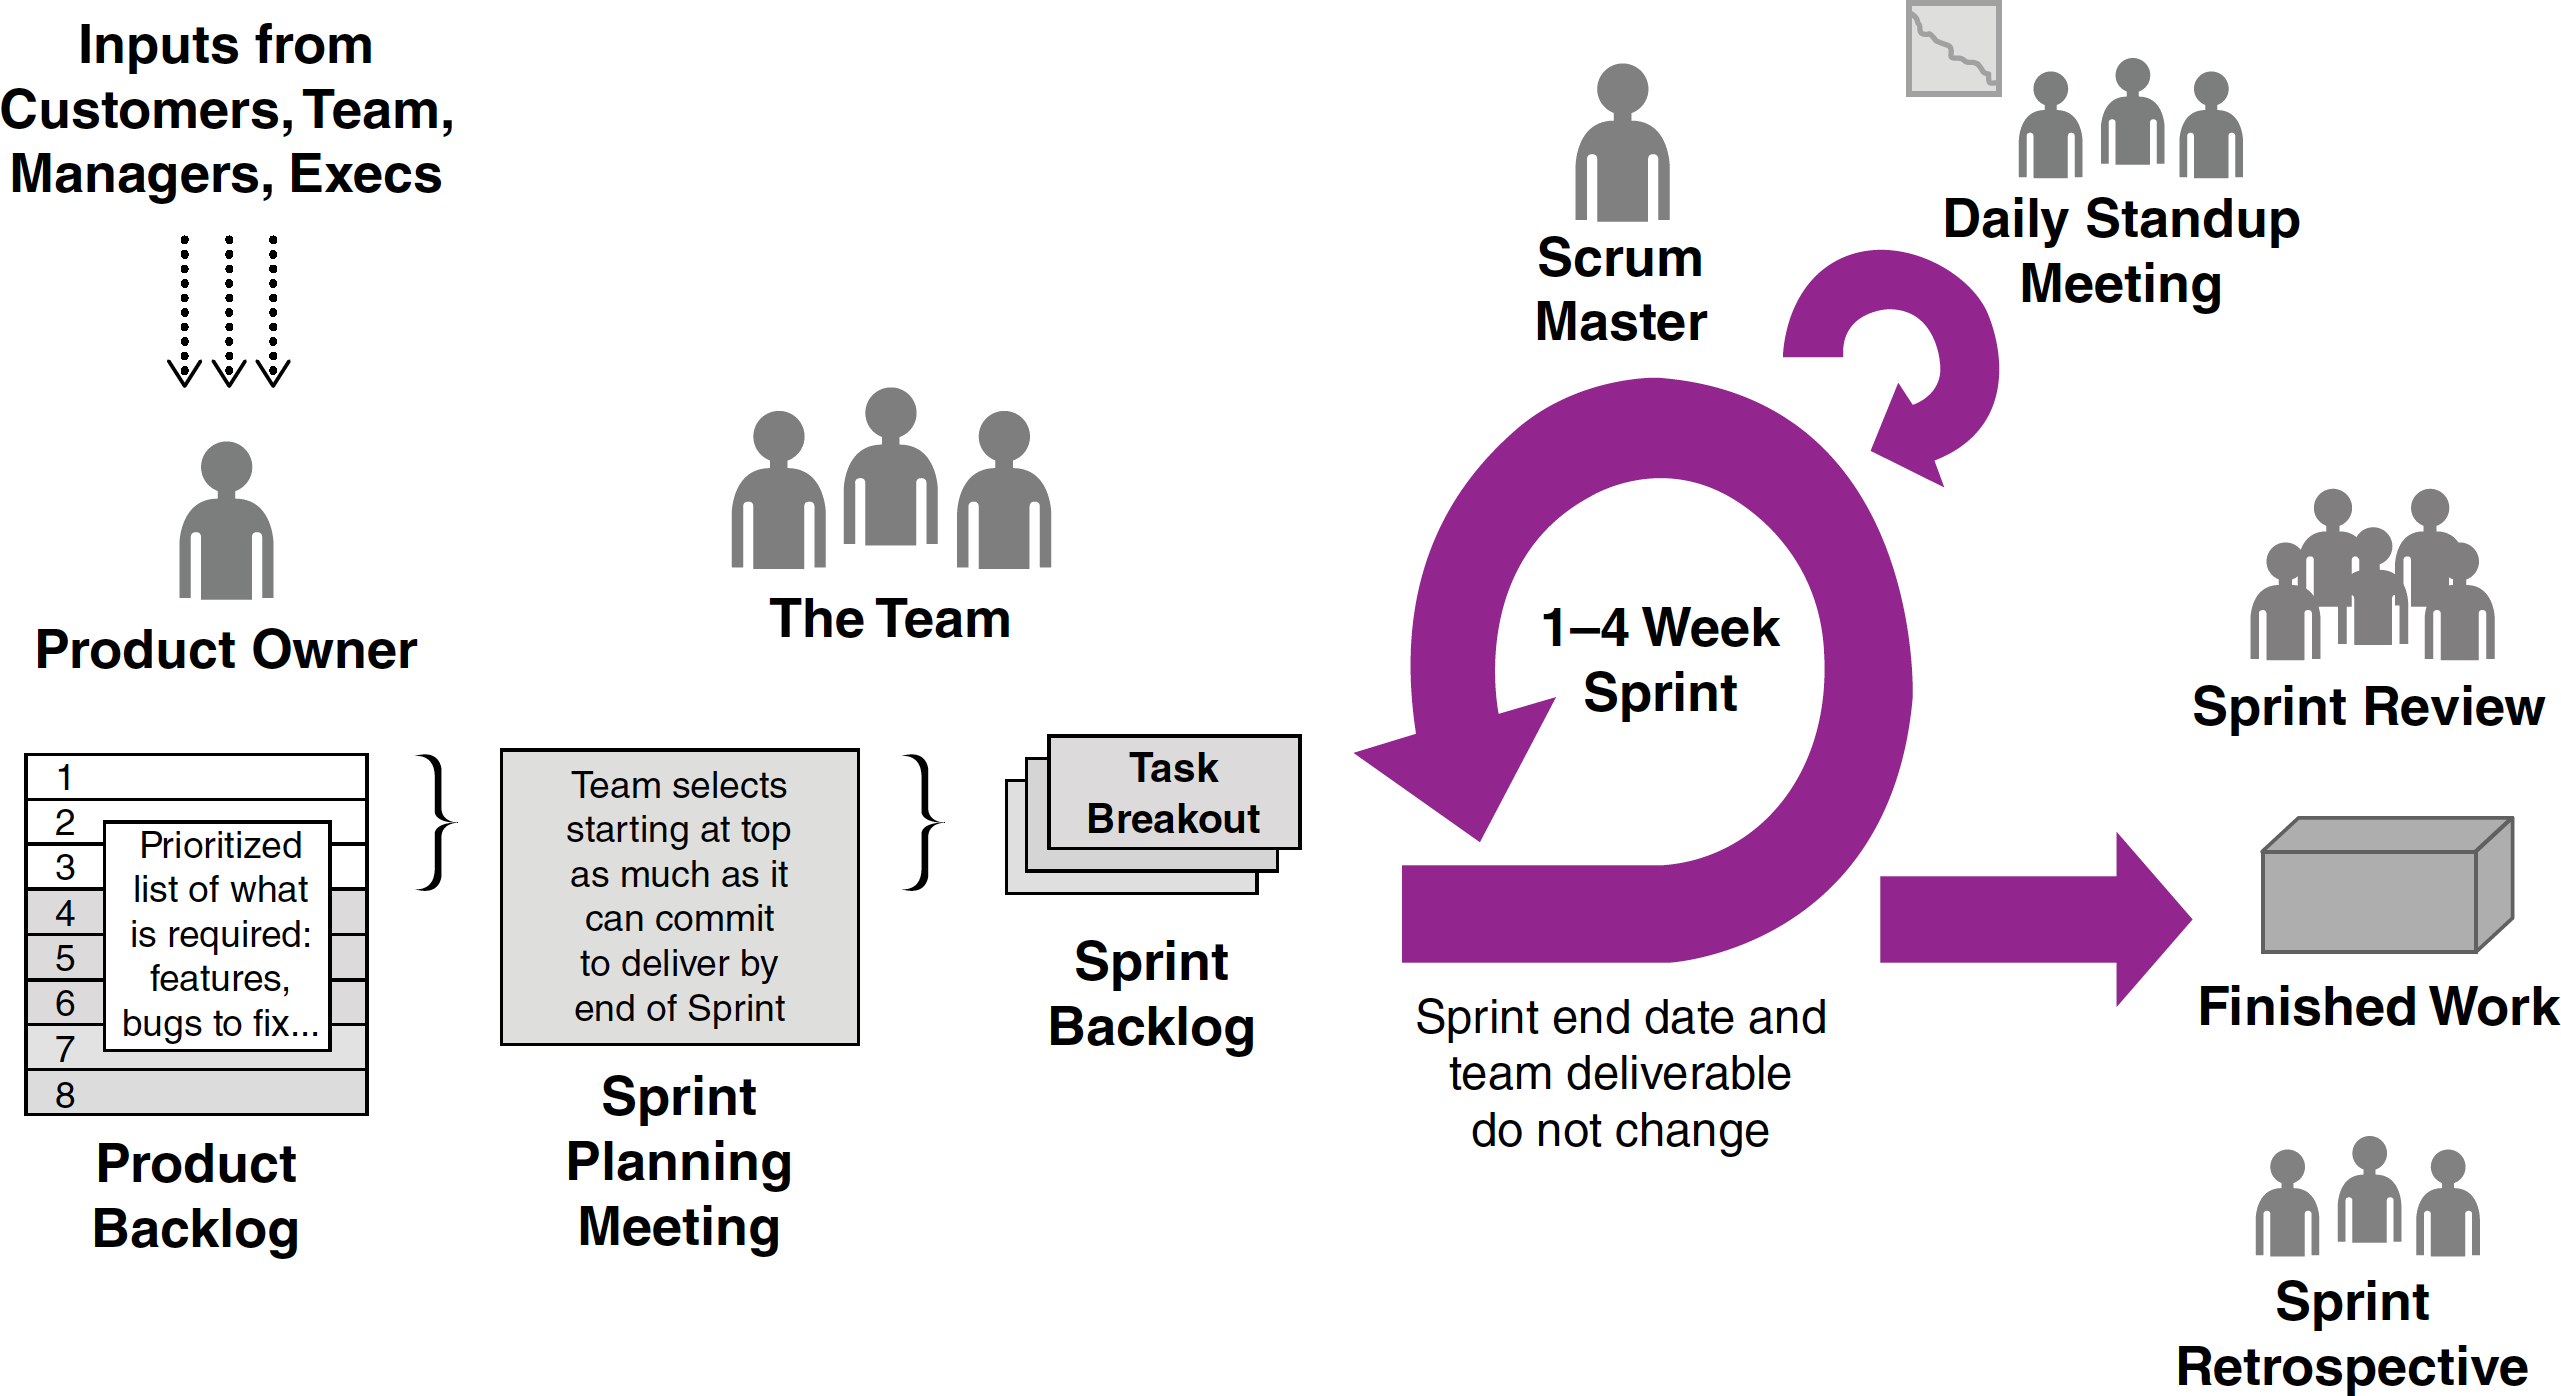
\includegraphics[width=125mm,scale=1]{Figuras/flujo_scrum}
% \caption{Flujo de la técnica SCRUM.}
%   \label{flujo_scrum}
% \end{figure}

\subsection{Planificación de iteraciones}
El primer día de la iteración se realiza la reunión de planificación de la iteración y consta de dos partes:
\begin{itemize}
    \item \textbf{Selección de requisitos} (4 horas máximo) – El PO presenta al equipo la lista de requisitos priorizada del producto o proyecto. El equipo pregunta al PO las dudas que surgen y selecciona los requisitos prioritarios que se compromete a completar en la iteración, de manera que puedan ser entregados en caso de ser solicitados.
    \item \textbf{Planificación de la iteración o sprint} (4 horas máximo) – El equipo elabora la lista de tareas de la iteración necesarias para desarrollar los requisitos a que se ha comprometido. La estimación de esfuerzo se hace de manera conjunta y los miembros del equipo se asignan las tareas.
\end{itemize}

\subsection{Ejecución del Sprint}
El equipo realiza una reunión diaria (15 minutos aproximadamente). Cada miembro del equipo inspecciona el trabajo que el resto está realizando (dependencias entre tareas, progreso hacia el objetivo de la iteración, obstáculos que pueden impedir este objetivo) para poder hacer las adaptaciones necesarias que permitan cumplir con el compromiso adquirido. En la reunión cada miembro del equipo responde a tres preguntas:
\begin{itemize}
    \item ¿Qué he hecho desde la última reunión diaria?
    \item ¿Qué voy a hacer a partir de este momento?
    \item ¿Qué impedimentos tengo o voy a tener?
\end{itemize}
Durante la iteración el Scrum Master se encarga de que el equipo pueda cumplir con su compromiso y de que no se merme la productividad del equipo. Además, elimina los obstáculos que el equipo no puede resolver por sí mismo.

Durante el sprint, el PO junto con el equipo refinen la lista de requisitos para prepararlos para los siguientes sprints y, si es necesario, cambian o vuelven a planificar los objetivos del proyecto para maximizar la utilidad de lo que se desarrolla y el retorno de inversión.

\subsection{Aporte}
En la tabla \ref{mis-aportes} se pueden apreciar los aportes propios en cada historia de usuario. El trabajo consistía en desarrollo de la historia, desarrollo de tests, y el miembro del equipo que no estuvo presente en el desarrollo de la historia es el encargado de hacer la validación de código y funcionalidad.

\begin{table}[H]
\centering
\small
\begin{tabular}{@{}ll@{}}
\toprule
Historias de usuario                                & Aporte \\ \midrule
Diseño de modelo de versionamiento de entidades     &  20\%  \\
Versionamiento de competencias                      & 61,5\% \\
Flujo de trabajo simple                             & 62,5\% \\
Aprobar pasos completados de flujos de trabajo      &  40\%  \\
Rechazar pasos completados de flujo de trabajo      &  60\%  \\
Buzón de entradas de flujos de trabajo              &  40\%  \\
Notificaciones con soporte a etapas                 &  20\%  \\
Versionamiento de evaluaciones                      & 37,5\% \\
Versionamiento de cursos                            & 61,5\% \\
Información básica de curso                         &  20\%  \\
Horas y unidades de evaluación de curso             &   8\%  \\
Especificaciones de curso                           &  40\%  \\
Requisitos de cursos                                &  60\%  \\
Revisar y aprobar curso                             &  40\%  \\
Competencias de curso                               &  25\%  \\
Esquema de curso                                    &  20\%  \\
Códigos de clasificación de curso                   &  60\%  \\
Información básica del programa                     &  50\%  \\
Competencias de programa                            &  60\%  \\
Bloques de curso por programa                       &  20\%  \\
Visualizar cambios en los campos                    &   8\%  \\
Roles de creación y edición para partes             &  23\%  \\
Diseño e implementación de etapas                   &  38\%  \\
Mejora en comportamientos para las etapas por roles & 37,5\% \\
Composición de etapas por roles                     &  23\%  \\
Etapas y partes opcionales por en la revisión       & 37,5\% \\
Notificaciones para las partes de flujos de trabajo &  20\%  \\
Reporte de esquemas de curso                        &  25\%  \\
Interfaz de alineación de códigos TOP/CIP           & 100\%  \\
Reorganización de pestañas del módulo curricular    & 100\%  \\
Lista mejorada de cursos y programas                & 100\%  \\
Retoques finales para el flujo de trabajo de curso  & 37,5\% \\ \bottomrule
\end{tabular}
\caption{Tabla de historias de usuario y aportes}
\label{mis-aportes}
\end{table}

Dichas historias de usuario eran entregadas para validación de parte del equipo de desarrolladores y por el equipo de expertos en didáctica, una vez que era aprobada se procedía a integrar el nuevo código en el repositorio.

\subsection{Inspección y adaptación}
El último día de la iteración se realiza la reunión de revisión del sprint la cual consta de dos partes:
\begin{itemize}
    \item \textbf{Demostración} (3 horas aproximadamente) – El equipo presenta al PO los requisitos completados en la iteración, en forma de incremento de producto preparado para ser entregado con el mínimo esfuerzo. En función de los resultados mostrados y de los cambios ocurridos en el contexto del proyecto, el PO realiza las adaptaciones necesarias de manera objetiva, ya desde la primera iteración, volviendo a planificar el proyecto.
    \item \textbf{Retrospectiva} (1 hora) - El equipo analiza cómo ha sido su manera de trabajar y cuáles son los problemas que podrían impedirle progresar adecuadamente, mejorando de manera continua su productividad. El Scrum Master se encargará de ir eliminando los obstáculos identificados.
\end{itemize}